%ieee
\documentclass[10pt]{IEEEtran}
\usepackage{amsmath}
\usepackage{cite}
\usepackage{ifthen}
\usepackage{seg}
\usepackage{color}
\usepackage{graphicx}
\usepackage{subfigure}

\DeclareRobustCommand{\dlo}[1]{}
\DeclareRobustCommand{\wen}[1]{#1}
\DeclareRobustCommand{\old}[1]{}
\DeclareRobustCommand{\new}[1]{#1}

\begin{document}

\end{document}


%ieee
\documentclass[12pt,journal,draftclsnofoot,onecolumn]{IEEEtran}
\usepackage{amsmath}
\usepackage{cite}
\usepackage{ifthen}
\usepackage{seg}
\usepackage{color}
\usepackage{graphicx}
\usepackage{subfigure}

\DeclareRobustCommand{\dlo}[1]{}
\DeclareRobustCommand{\wen}[1]{#1}
\DeclareRobustCommand{\old}[1]{}
\DeclareRobustCommand{\new}[1]{#1}

\begin{document}

\end{document}


%geophysics
\documentclass[manuscript,revised]{geophysics}
\usepackage{amsmath}

\begin{document}

\end{document}

%JAG

\documentclass[preprint,amsmath,authoryear,12pt,manuscript]{elsarticle}
\usepackage{amsmath}
\usepackage{lineno}
\usepackage{graphicx}
\usepackage{subfigure}
\usepackage{setspace}
\usepackage{ulem}
\usepackage{color}
\usepackage{morefloats}

\DeclareRobustCommand{\dlo}[1]{}
\DeclareRobustCommand{\wen}[1]{#1}
\DeclareRobustCommand{\old}[1]{}
\DeclareRobustCommand{\new}[1]{#1}
\journal{Computers and Geosciences}
\linenumbers
\doublespacing
\begin{document}

\end{document}



%\AtEndDocument{}

%\newpage
%\listoffigures




#two columns
Paper('ieee',lclass='IEEEtran',options='10pt',use='ulem,cite,ifthen,seg,color,graphicx,subfigure,amsmath')

#one column
Paper('ieee_one',lclass='IEEEtran',options='12pt,journal,draftclsnofoot,onecolumn',use='cite,ifthen,seg,color,graphicx,subfigure,amsmath,epstopdf')

#revision 1
#two columns
Paper('ieee_r1',lclass='IEEEtran',options='10pt',use='ulem,cite,ifthen,seg,color,graphicx,subfigure,amsmath',include=r'''
\DeclareRobustCommand{\old}[1]{\color{blue}{\sout{#1}}\color{black}{}}
\DeclareRobustCommand{\new}[1]{\color{red}{\textit{#1}}\color{black}{}} 
''')

Command('ieee_p1.tex','ieee_r1.tex','cp $SOURCE $TARGET')
Paper('ieee_p1',lclass='IEEEtran',options='10pt',use='cite,ifthen,seg,color,graphicx,subfigure,amsmath',include=r'''
\DeclareRobustCommand{\old}[1]{}
\DeclareRobustCommand{\new}[1]{#1}
''')

#one column
Paper('ieee_one_p1',lclass='IEEEtran',options='12pt,journal,draftclsnofoot,onecolumn',use='cite,ifthen,seg,color,graphicx,subfigure,amsmath,epstopdf',include=r'''
\DeclareRobustCommand{\old}[1]{}
\DeclareRobustCommand{\new}[1]{#1}
\DeclareRobustCommand{\dlo}[1]{}
\DeclareRobustCommand{\wen}[1]{#1}
''')


#revision 2
#two columns
Paper('ieee_r2',lclass='IEEEtran',options='10pt',use='ulem,cite,ifthen,seg,color,graphicx,subfigure,amsmath',include=r'''
\DeclareRobustCommand{\dlo}[1]{}
\DeclareRobustCommand{\wen}[1]{#1}
\DeclareRobustCommand{\old}[1]{\color{blue}{\sout{#1}}\color{black}{}}
\DeclareRobustCommand{\new}[1]{\color{red}{\textit{#1}}\color{black}{}} 
''')

Command('ieee_p2.tex','ieee_r2.tex','cp $SOURCE $TARGET')
Paper('ieee_p2',lclass='IEEEtran',options='10pt',use='cite,ifthen,seg,color,graphicx,subfigure,amsmath',include=r'''
\DeclareRobustCommand{\dlo}[1]{}
\DeclareRobustCommand{\wen}[1]{#1}
\DeclareRobustCommand{\old}[1]{}
\DeclareRobustCommand{\new}[1]{#1}
''')

#one column
Paper('ieee_one_p1',lclass='IEEEtran',options='12pt,journal,draftclsnofoot,onecolumn',use='cite,ifthen,seg,color,graphicx,subfigure,amsmath,epstopdf',include=r'''
\DeclareRobustCommand{\old}[1]{}
\DeclareRobustCommand{\new}[1]{#1}
\DeclareRobustCommand{\dlo}[1]{}
\DeclareRobustCommand{\wen}[1]{#1}
''')

env=Environment()
env.Command(['ieee','IEEEtran.bst','IEEEtran.cls'],[os.getenv('HOME')+'/chenyk.open/temp/ieee/IEEEtran.bst',os.getenv('HOME')+'/chenyk.open/temp/ieee/IEEEtran.cls'],'cp  ${SOURCES[0]}  ${TARGETS[1]} && cp  ${SOURCES[1]}  ${TARGETS[2]} ')








%\listoffigures

%\AtEndDocument{
%\begin{figure}[htb!]
%  \centering
%  \subfloat[]{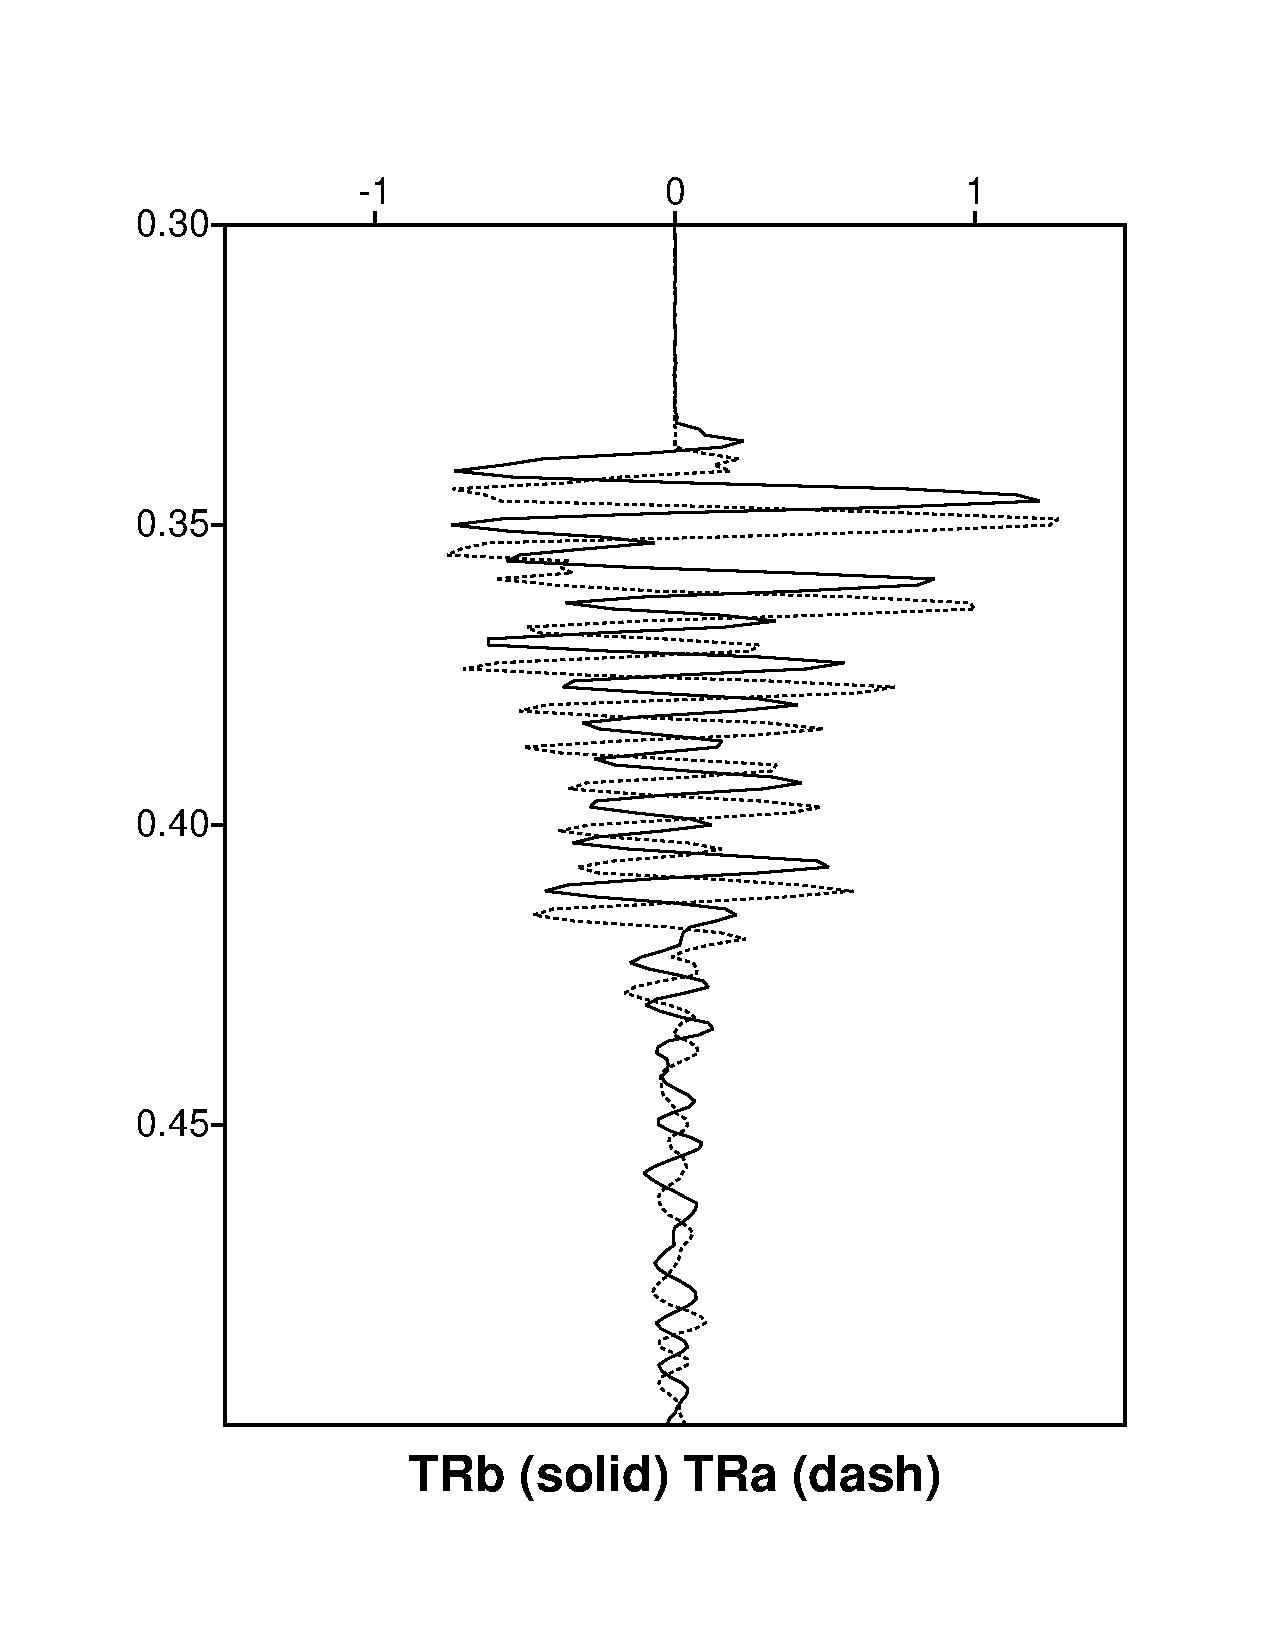
\includegraphics[width=0.45\textwidth]{path/Fig/fig1}
%    \label{fig:fig1}}
%  \subfloat[]{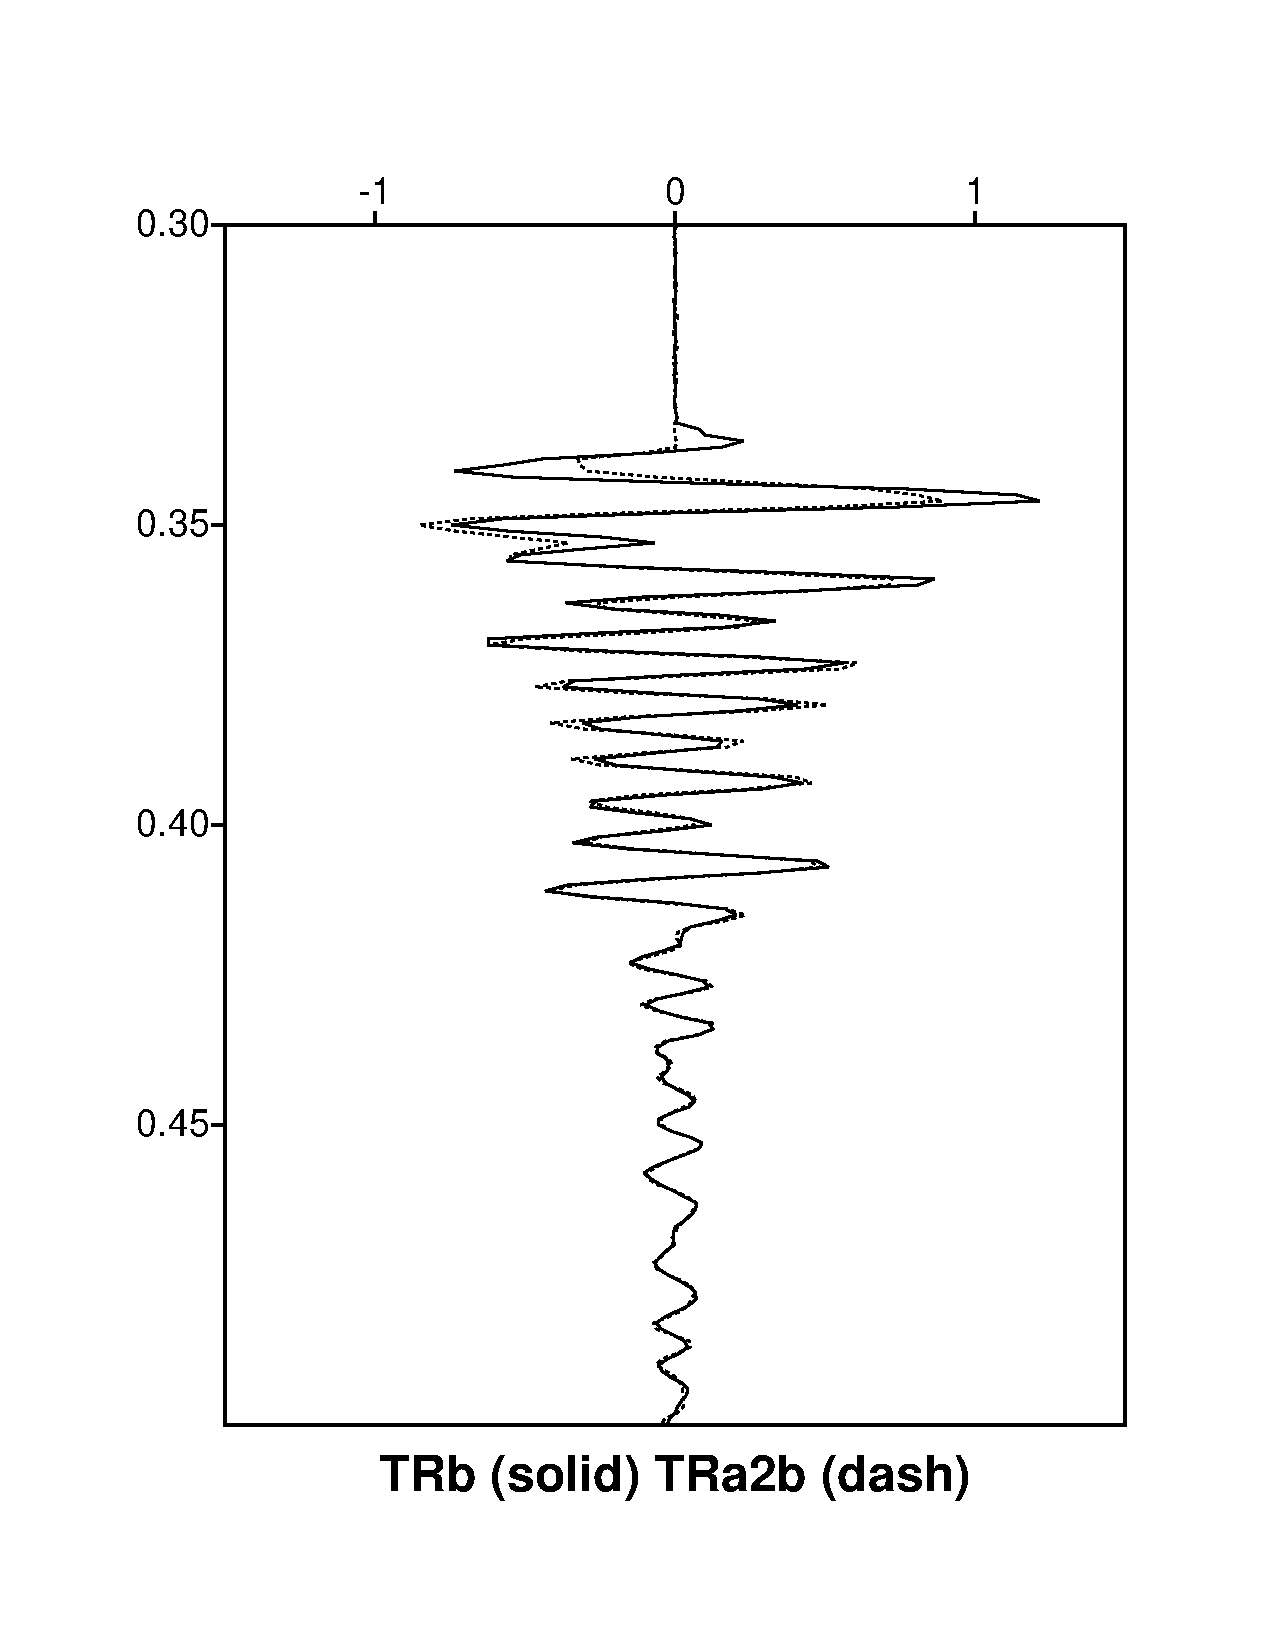
\includegraphics[width=0.35\textwidth]{path/Fig/fig2}
%    \label{fig:fig2}}    
%   \caption{caption goes here}
%   \label{fig:fig1,fig2}
%\end{figure}

%\begin{figure*}[ht!]
%  \centering
%  \subfloat[]{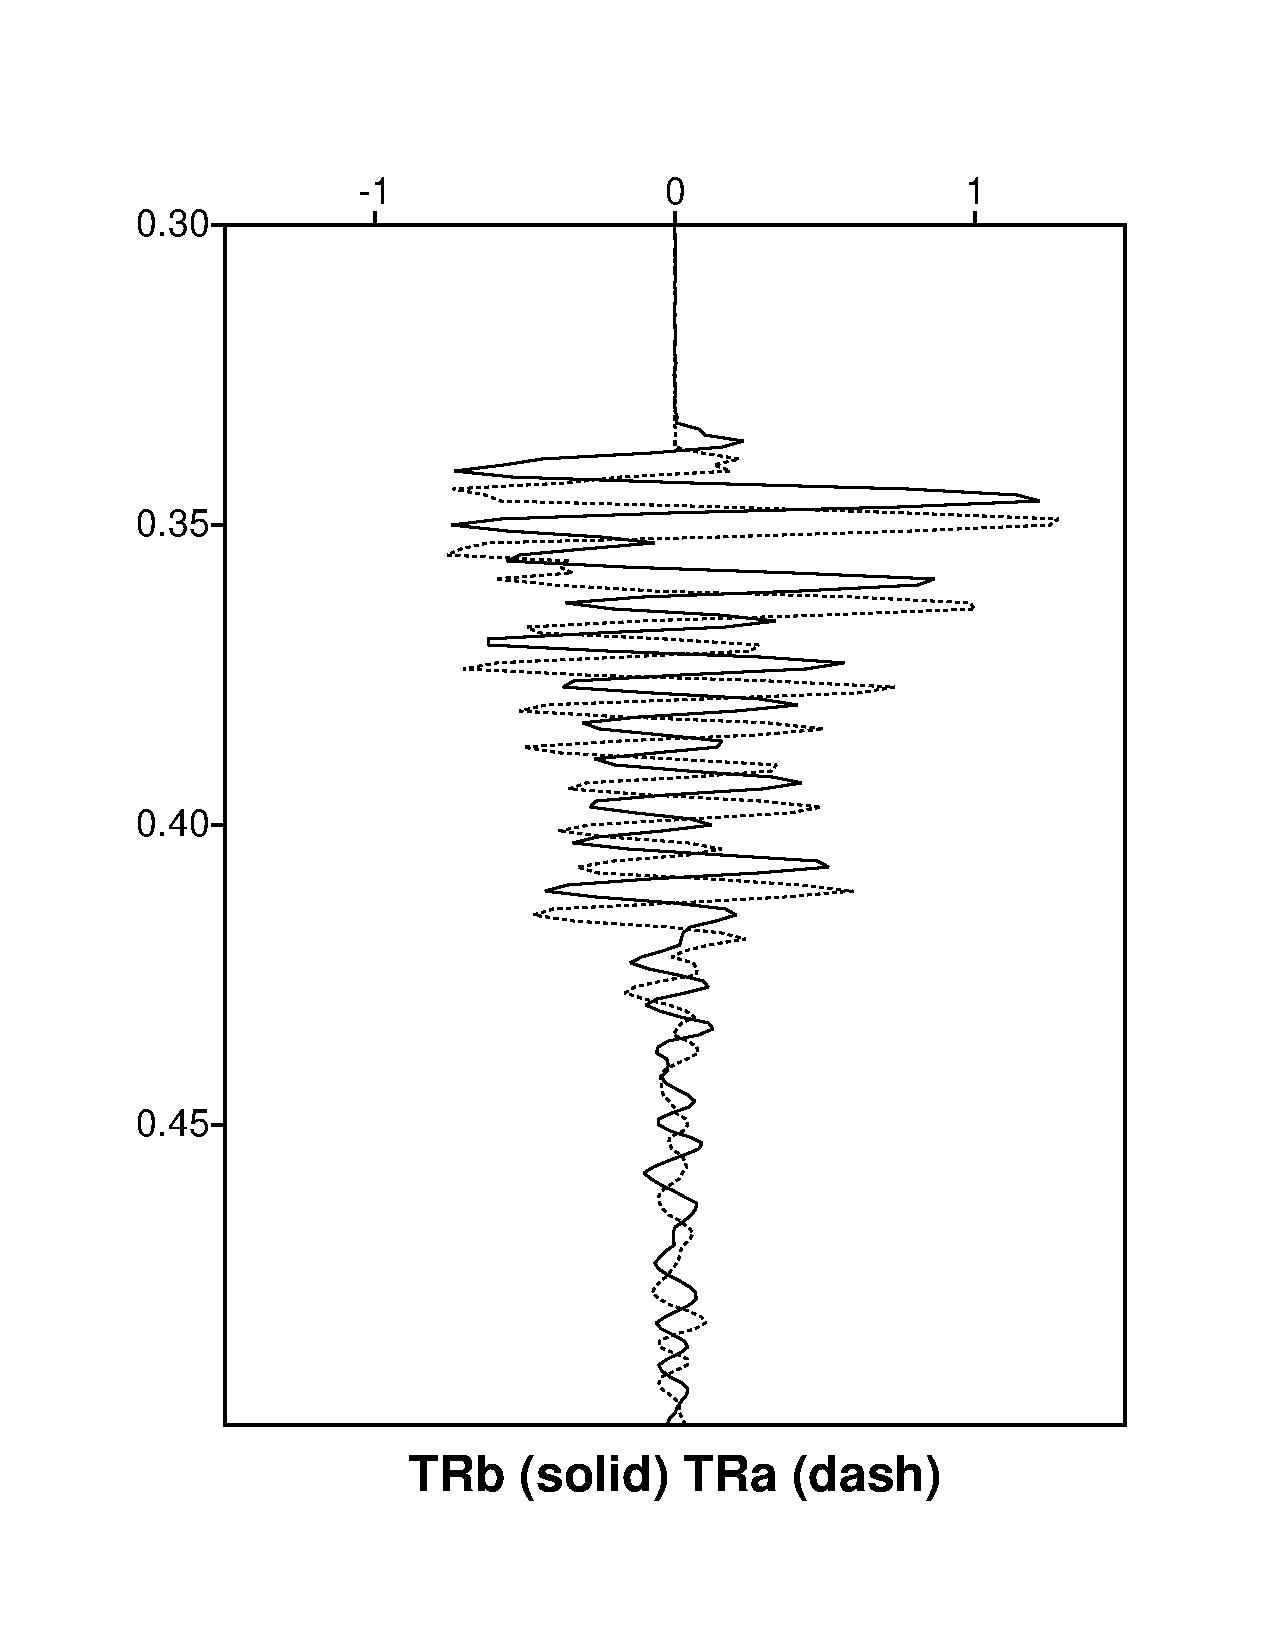
\includegraphics[width=0.45\textwidth]{path/Fig/fig1}
%    \label{fig:fig1}}
%  \subfloat[]{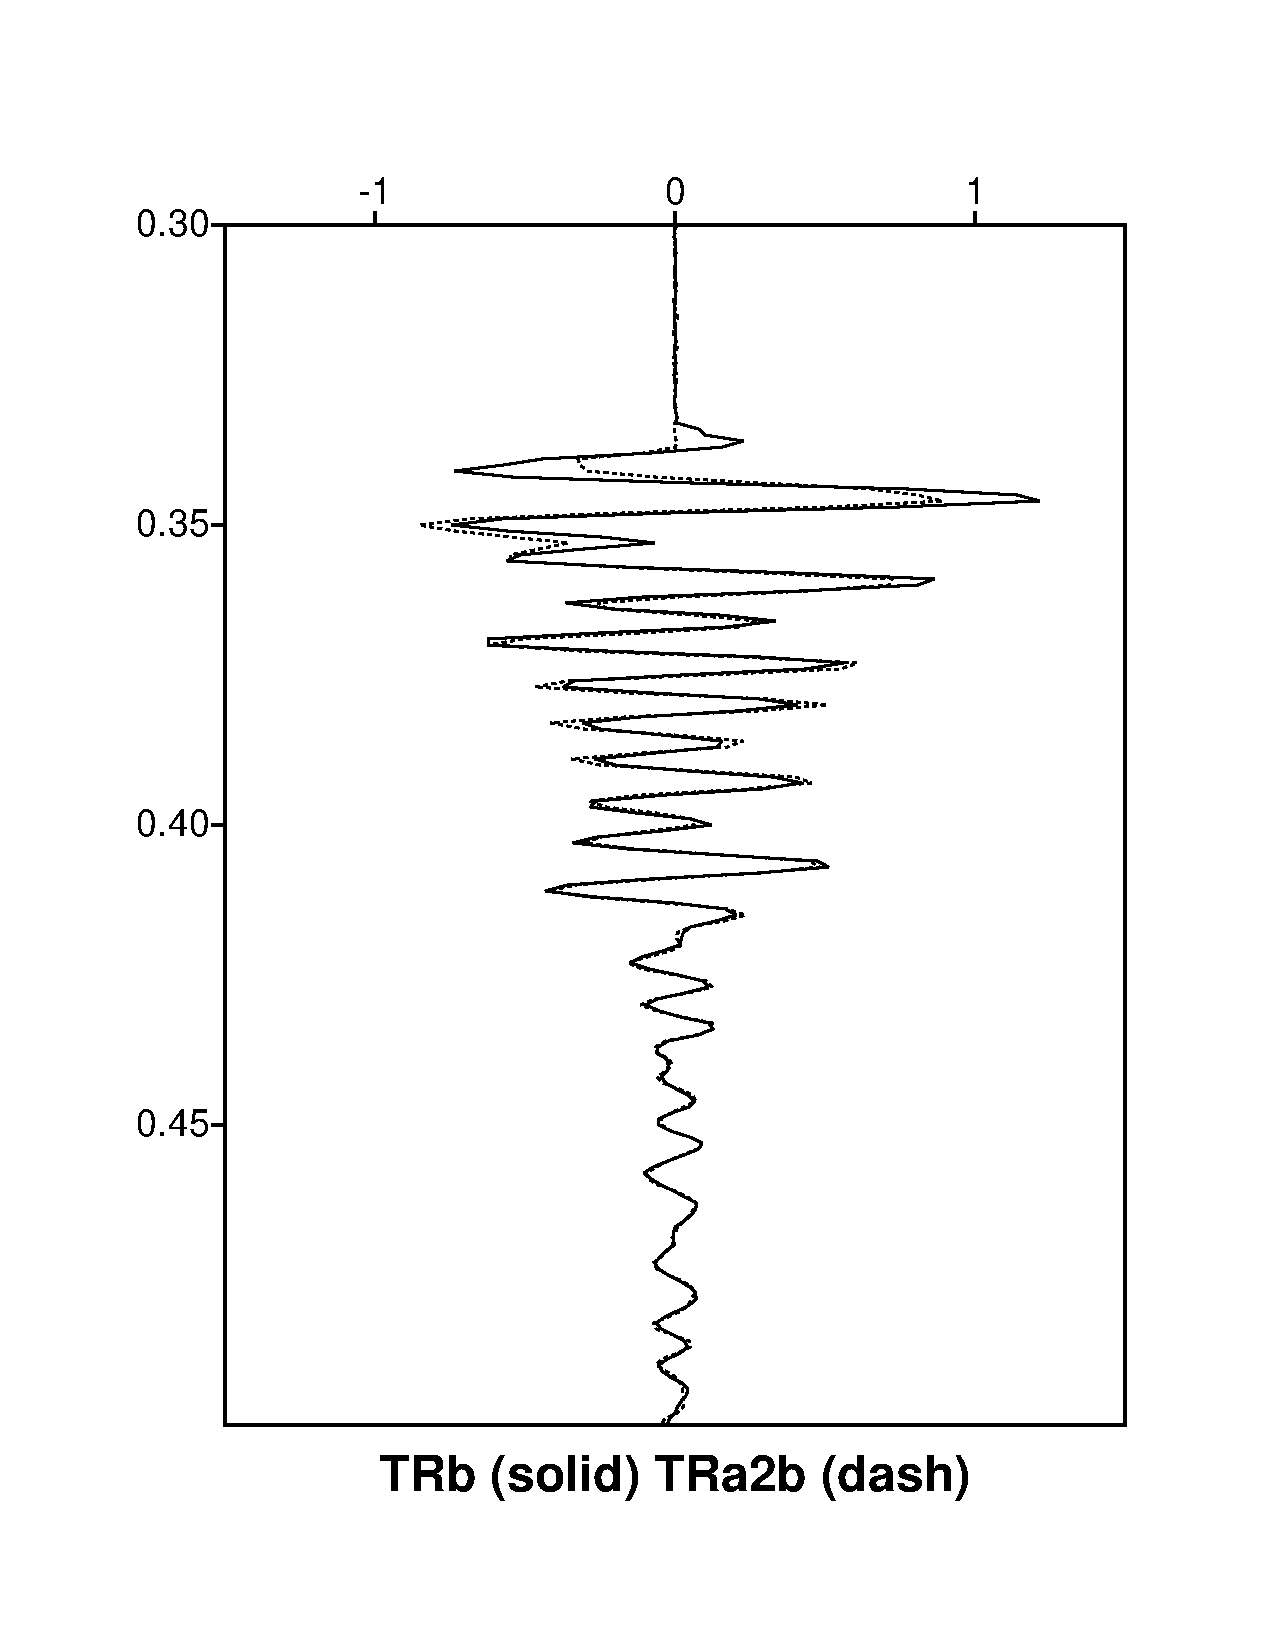
\includegraphics[width=0.35\textwidth]{path/Fig/fig2}
%    \label{fig:fig2}}    
%   \caption{caption goes here}
%   \label{fig:fig1,fig2}
%\end{figure*}

%\begin{figure*}[ht!]
%  \centering
%  \subfigure[]{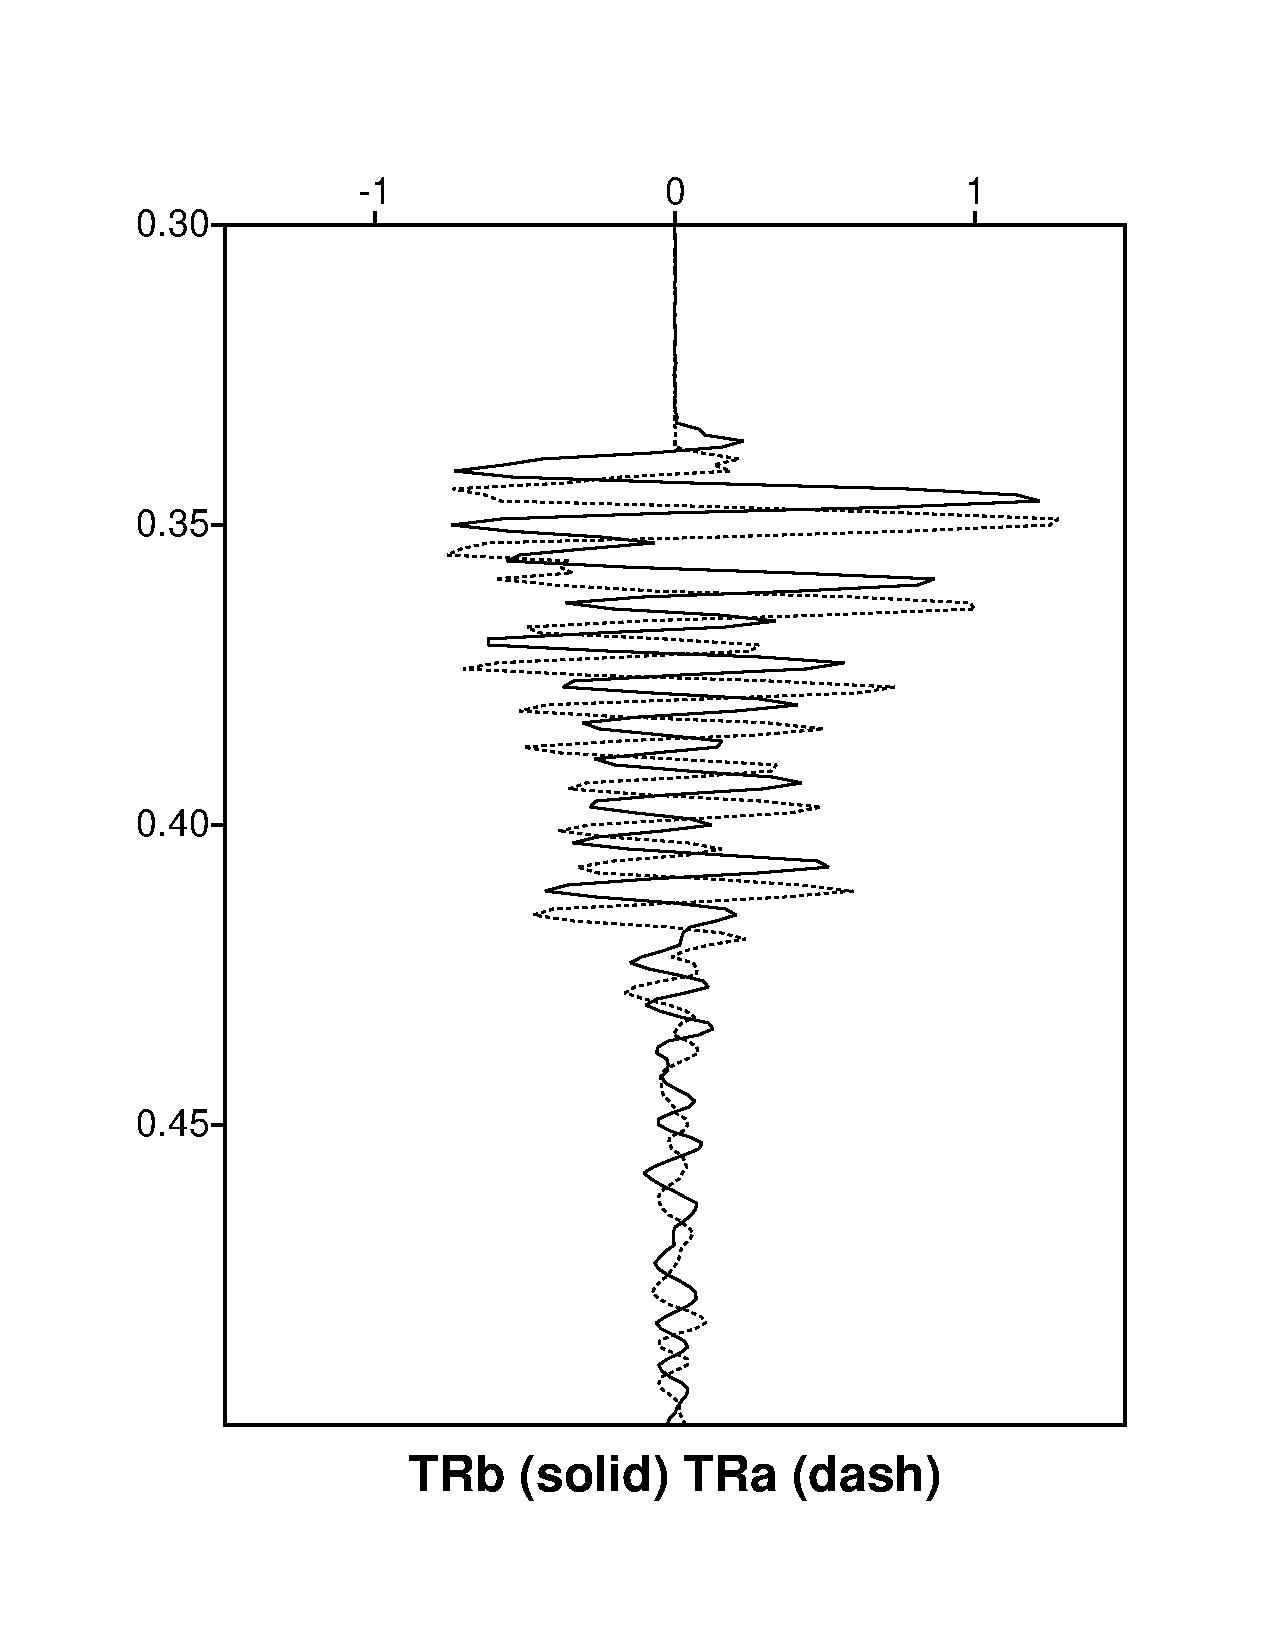
\includegraphics[width=0.45\textwidth]{path/Fig/fig1}
%    \label{fig:fig1}}
%  \subfigure[]{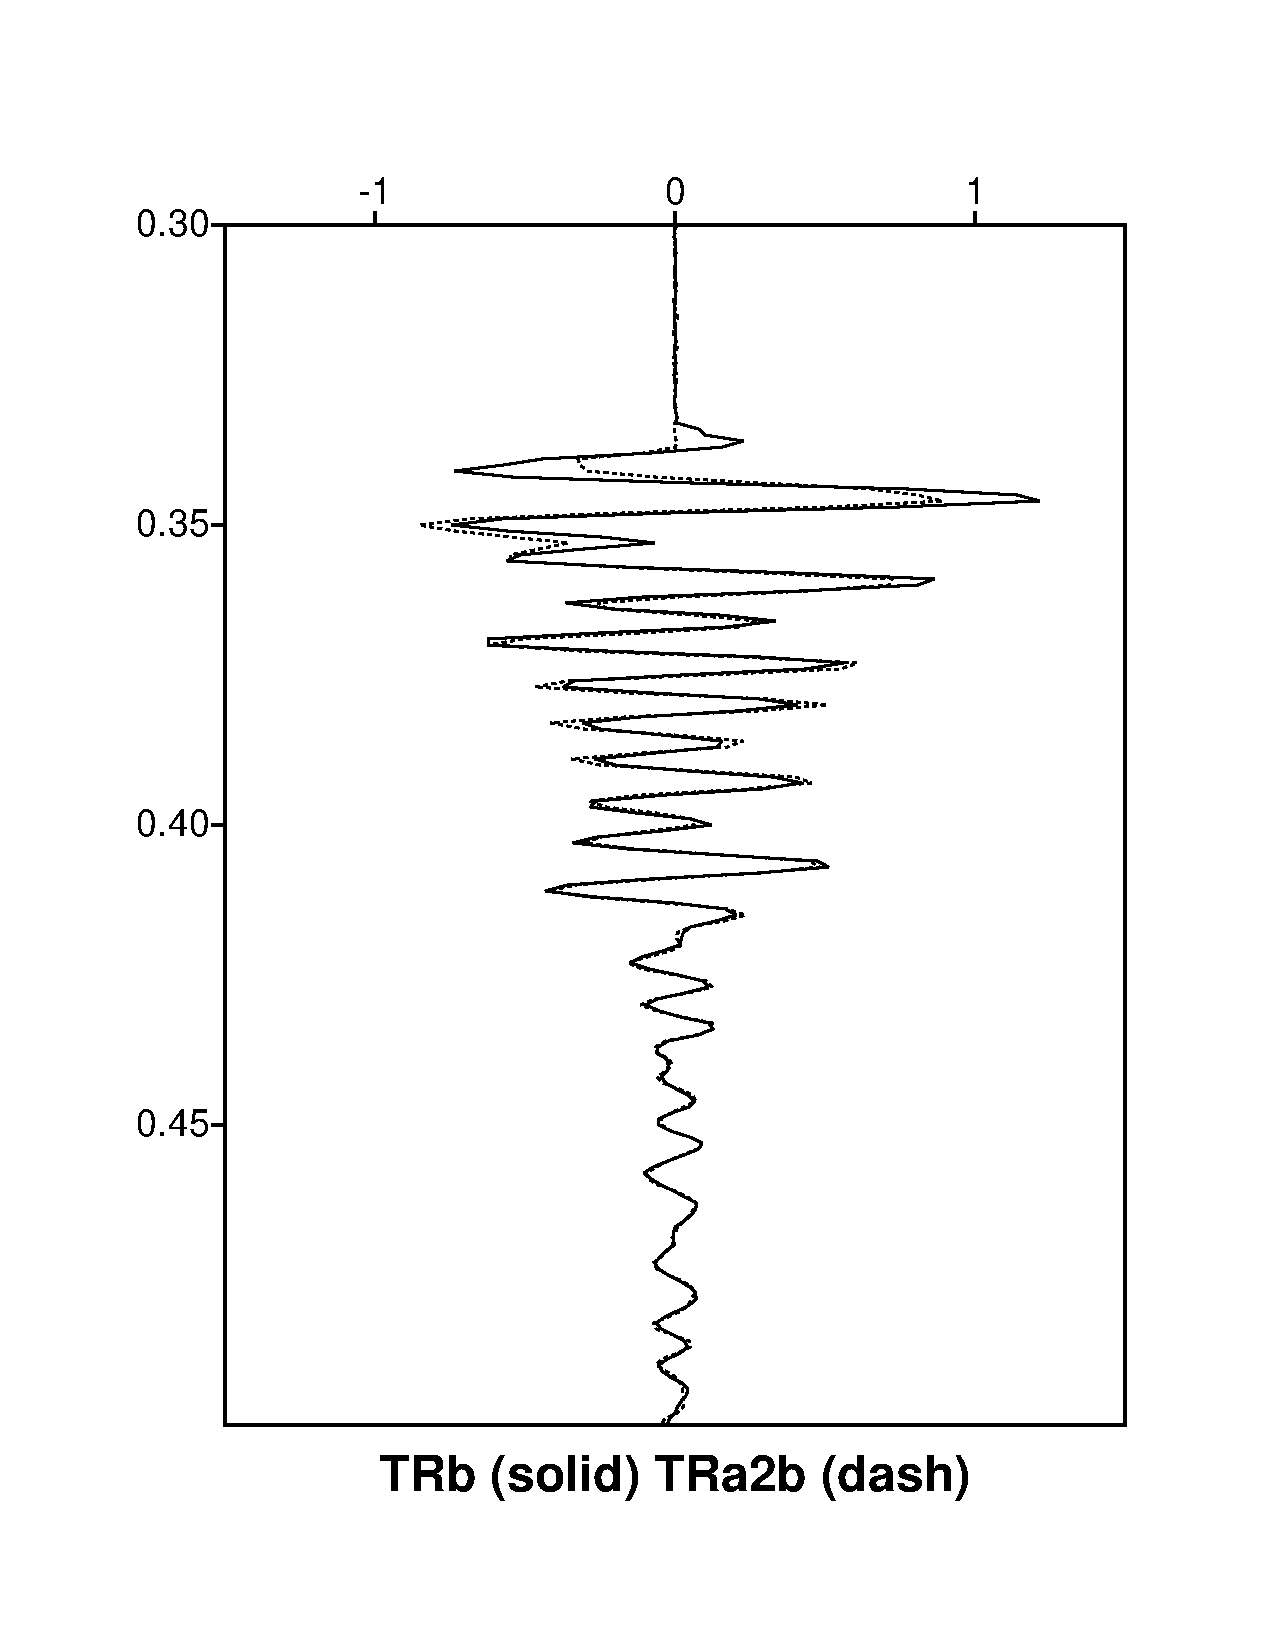
\includegraphics[width=0.35\textwidth]{path/Fig/fig2}
%    \label{fig:fig2}}    
%   \caption{caption goes here}
%   \label{fig:fig1,fig2}
%\end{figure*}


%\begin{figure}[htb!]
%  \centering
%  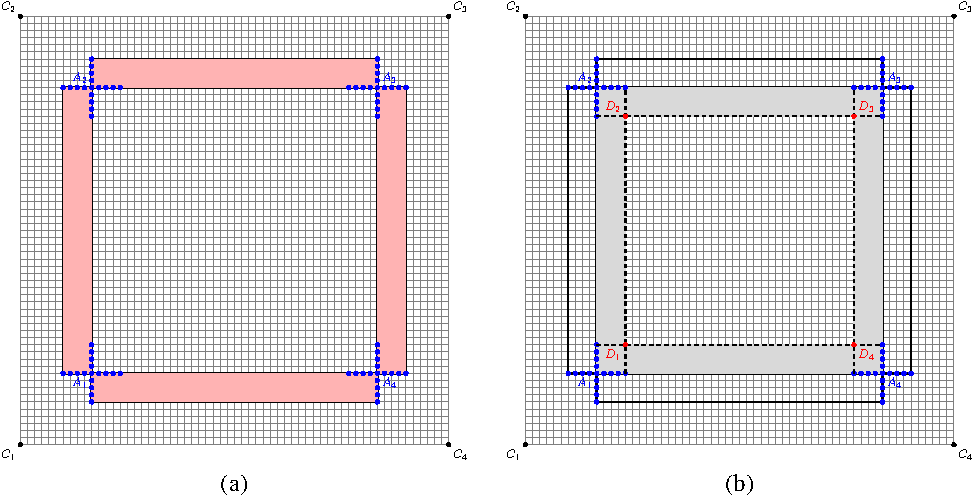
\includegraphics[width=0.45\textwidth]{path/Fig/fig3}
%   \caption{caption goes here}
%   \label{fig:fig3}
%\end{figure}
%}
%\newpage
%\listoffigures


%\begin{table}[h]
%\caption{Table caption}
%\begin{center}
%     \begin{tabular}{|c|c|c|c|c|c|} 
%	  \hline Column1 (unit)  & Column2 (unit) & Column3 (unit) \\ 
%	  \hline 1 & 2  & 3 \\
%       \hline
%    \end{tabular} 
%\end{center}
%\label{tbl:table1}
%\end{table}



